%-------------------------------------------------------------------------------
% seq64_midi_formats
%-------------------------------------------------------------------------------
%
% \file        seq64_midi_formats.tex
% \library     Documents
% \author      Chris Ahlstrom
% \date        2015-09-03
% \update      2015-11-25
% \version     $Revision$
% \license     $XPC_GPL_LICENSE$
%
%     Provides a discussion of the formats (legacy and new) of the last
%     track of an Seq24/Sequencer64 MIDI file.
%
%-------------------------------------------------------------------------------

\section{MIDI Format and Other MIDI Notes}
\label{sec:midi_format_and_midi_notes}

\subsection{Standard MIDI Format 0}
\label{subsec:midi_format_smf_0}

   \textbf{New:}
   \index{new!smf 0 support}
   \index{new!channel split}
   \textsl{Sequencer64} can now read and import SMF 0 MIDI files, and performs
   channel splitting automatically.

   When an SMF 0 format is detected, \textsl{Sequencer64}
   reads the file as if were an SMF 1 file, but puts all of the events into the
   same sequence/pattern.  While the file is being processed, a list of the
   channels present in the track is maintained.

   Once the end-of-track is encountered for that sequence, one new empty
   sequence is created for each channel found in the original (main) sequence.
   The events in the main sequence are scanned, one by one, and added at the
   end of the appropriate sequence.  If the event is a channel event,
   then the event is inserted into the sequence that was created for that
   channel.  If the event is a non-channel event, then each sequence gets a
   copy of that event.

   After processing, the MIDI buss information, track name, and other pieces of
   information are attached to each sequence.  The following figure shows in
   imported SMF 0 tune, split into tracks.

\begin{figure}[H]
   \centering 
   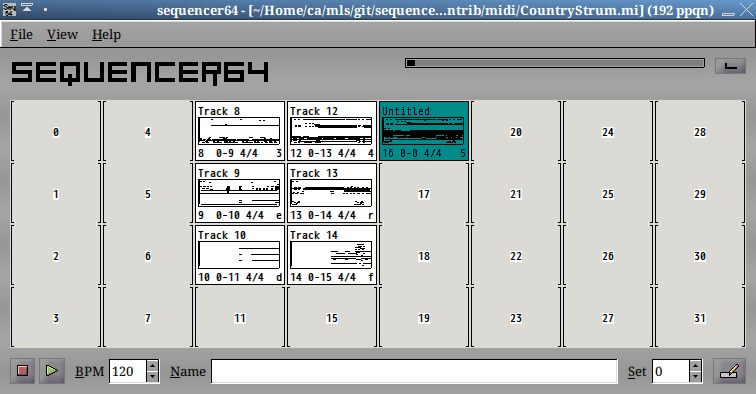
\includegraphics[scale=0.75]{smf0/imported-smf-0-song.png}
   \caption{Imported SMF 0 MIDI Song}
   \label{fig:imported_smf_0_song}
\end{figure}

   The original imported SMF 0 track is preserved, intact, in main window
   pattern slot \#16.  It is highlighted in a dark cyan color to remind the
   user that it is not a playable sequence.  It has no channel number.  It is
   assigned the non-existent MIDI channel of 0.  If the original track had no
   title, this track is named "Untitled".  Normally, one will either delete
   this track before saving the file, or at least keep it muted.

   Each new, single-channel track is given a title of either the form
   "N: Track-name" or, if the song was untitled, "Track N".
   The sequence number of each new track is the internal channel number (which
   is always the actual MIDI channel number minus one).

   The time-signature of each track is currently set to defaults.

   \textbf{TODO:}
   \index{todo!tempo events}
   \index{todo!time signature events}
   In the future, we will add support for obtaining some of the other
   information a MIDI SMF 0 track might have, such as the Tempo and the
   Time Signature.

   The original SMF 0 track is also shown in the song editor, as shown in the
   following figure.

\begin{figure}[H]
   \centering 
   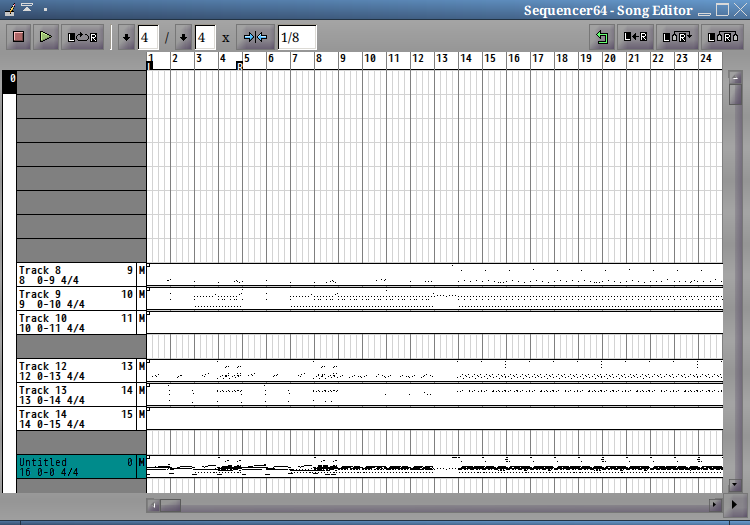
\includegraphics[scale=0.75]{smf0/imported-smf-0-song-editor.png}
   \caption{SMF 0 MIDI Song in the Song Editor}
   \label{fig:imported_smf_0_song_editor}
\end{figure}

   One is free to edit the imported tune to heart's content.
   Here, we added one instance of each track, including the SMF 0 track,
   to show what the imported song looks like.

\subsection{Legacy Proprietary Track Format}
\label{subsec:legacy_midi_format}

   The authors of \textsl{Seq24} took the trouble to make sure that the format
   of the MIDI files it write are compatible with other MIDI applications.
   \textsl{Seq24} also stores its own information (triggers, MIDI control
   information, etc) in the file, but marked so that other sequencers can read
   the file and ignore the \textsl{Seq24}-specific information.

   \textsl{Sequencer64} continues that MIDI-compliant behavior, but has
   improved the compliance just a little bit. 

   We call that last chunk of sequencer-specific information the "proprietary
   track".

   Before we discuss that last, proprietary track, note that the normal MIDI
   tracks that
   precede it include the SeqSpec ("sequencer-specific", sort of)
   control tags shown in \tableref{table:seqspec_items_normal_tracks}.
   These control tags are global constants in the \textsl{Seq24} source
   code, ranging from 0x24240001 to 0x24240013.

   \begin{table}[htb]
      \centering
      \caption{SeqSpec Items in Normal Tracks}
      \label{table:seqspec_items_normal_tracks}
      \begin{tabular}{l l}
         \texttt{c\_midibus}        & \texttt{24 24 00 01 00 00 00 00} \\
         \texttt{c\_midich}         & \texttt{24 24 00 02 00 00 00 00} \\
         \texttt{c\_triggers}       & \texttt{24 24 00 04 00 00 00 00} \\
         \texttt{c\_timesig}        & \texttt{24 24 00 06 00 00 00 00} \\
         \texttt{c\_triggers\_new}  & \texttt{24 24 00 08 00 00 00 00} \\
         \texttt{c\_musickey}       & \texttt{24 24 00 11 00} \\
         \texttt{c\_musicscale}     & \texttt{24 24 00 12 00} \\
         \texttt{c\_backsequence}   & \texttt{24 24 00 13 00 00 00 00} \\
      \end{tabular}
   \end{table}

   The \texttt{c\_triggers} tag is obsolete.

   \textbf{New:}
   \index{new!saved control tags}
   The \texttt{c\_musickey},
   \texttt{c\_musicscale}, and
   \texttt{c\_backsequence}
   control tags are new with \textsl{Sequencer64} v. 0.9.9.7.
   They are now saved as additional information in each sequence in which they
   have been specified in the sequence editor.
   However, for backward compatibility (and because it is probably the more
   common use case), these items can also be
   saved globally for the whole MIDI song, as an option.

   Note that these tags (created by the application, but not present in the
   proprietary track, and perhaps also created by other MIDI applications) are
   preceded by the standard MIDI "FF 7F length" meta-event sequence.

   The following discussion applies to the final "proprietary" track as
   saved in the legacy \textsl{Seq24} format.

   After all the counted MIDI tracks are read, \textsl{Seq24} checks for
   extra data.  If there is extra data, \textsl{Seq24} reads a long value.
   The first one encountered is a MIDI "sequencer-specific"
   (\textsl{SeqSpec}) section.  It starts with

   \begin{verbatim}
      0x24240010 == a Seq24 c\_midictrl proprietary value
   \end{verbatim}

   Getting this value first is simplified MIDI in two ways.
   First, the second does not begin with any kind of track marker.  MIDI
   requires an "MTrk" marker to start a track, though it also requires
   unknown markers to be supported.  Some applications, like
   \textsl{timidity}, handle this situation.  Others, like \textsl{midicvt},
   complain about an unexpected header marker.
   Second, normally, MIDI wants to see the triad of

   \begin{verbatim}
      status = FF, type= 7F (proprietary), length = whatever
   \end{verbatim}

   to precede proprietary data.
   Now, as shown by \tableref{table:midi_file_support_table},
   most applications accept the shortcut legacy format, but \textsl{midicvt}
   does not.

   So, as a "bug" fix, we now write and read
   this information properly in \textsl{Sequencer64}; it is now
   preceded by the \texttt{0xFF 0x7F} marker..
   We also need to be able to read legacy Seq24 MIDI files, so that ability has
   been preserved in \textsl{Sequencer64}..

   Anyway, at this point, we have the \textbf{c\_midictrl} information now.
   Next, we read a long value, seqs.  It is 0.

   \begin{verbatim}
      24 24 00 10 00 00 00 00
   \end{verbatim}

   Read the next long value, 0x24240003.  This is \textbf{c\_midiclocks}.
   We get a value of 0 for "TrackLength" (now a local variable called
   "busscount"):

   \begin{verbatim}
      24 24 00 03 00 00 00 00
   \end{verbatim}

   If the buss-count was greater than 0, then for each value, we would read a
   byte value represent the bus a clock was on, and setting the clock value
   of the master MIDI buss.
   Another check for more data is made.

   \begin{verbatim}
      24 24 00 05 00 20 00 00
   \end{verbatim}

   0x24240005 is \textbf{c\_notes}.  The value screen\_sets is read (two
   bytes) and
   here is 0x20 = 32.  For each screen-set:

   \begin{verbatim}
      len = read\_short()
   \end{verbatim}

   If non-zero, each of the \texttt{len} bytes is appended as a string.
   Here, len is 0 for all 32 screensets, so the screen-set notepad is set to
   an empty string.
   Another check for more data is made.

   \begin{verbatim}
      24 24 00 07 00 00 00 78
   \end{verbatim}

   0x24240007 is \textbf{c\_bpmtag}.  The long value is read and sets the
   perform object's bpm value.  Here, it is 120 bpm.
   Another check for more data is made.

   \begin{verbatim}
      24 24 00 09 00 00 04 00
   \end{verbatim}

   0x24240009 is \textbf{c\_mutegroups}.  The long value obtained here is
   1024.  If this value is not equal to the constant
   \textbf{c\_gmute\_tracks} (1024), a warning is emitted to the console,
   but processing continues anyway, 32 x 32 long values are read to select
   the given group-mute, and then set each of its 32 group-mute-states.

   In our sample file, 32 groups are specified, but all 32 group-mute-state
   values for each are 0.

   So, to summarize the legacy proprietary track's data, ignoring the data
   itself, which is mostly 0 values, as shown in
   \tableref{table:seqspec_items_legacy_track}

   \begin{table}[htb]
      \centering
      \caption{SeqSpec Items in Legacy Proprietary Track}
      \label{table:seqspec_items_legacy_track}
      \begin{tabular}{l l}
\texttt{c\_midictrl}    & \texttt{24 24 00 10 00 00 00 00} \\
\texttt{c\_midiclocks}  & \texttt{24 24 00 03 00 00 00 00} (buss count = 0) \\
\texttt{c\_notes}       & \texttt{24 24 00 05 00 20 00 00} (screen sets = 32) \\
\texttt{c\_bpmtag}      & \texttt{24 24 00 07 00 00 00 78} (bpm = 120) \\
\texttt{c\_mutegroups}  & \texttt{24 24 00 09 00 00 04 00} (mg = 1024) \\
      \end{tabular}
   \end{table}

   The new format (again, ignoring the data) takes up a few more bytes.
   It starts with the normal track marker and size data, followed by a
   made-up track name ("Sequencer64-S"),
   as shown in \tableref{table:seqspec_items_new_track}.

   \begin{table}[htb]
      \centering
      \caption{SeqSpec Items in New Proprietary Track}
      \label{table:seqspec_items_new_track}
      \begin{tabular}{l l}
\texttt{"MTrk" etc.}   & \texttt{4d 54 72 6b 00 00 11 0d 00 ...} \\
\texttt{Track name}    & \texttt{53 65 71 75 65 6e 63 65 72 32 34 2d 53} \\
\texttt{c\_midictrl}   & \texttt{ff 7f 04 24 24 00 10 00} (???) \\
\texttt{c\_midiclocks} & \texttt{ff 7f 04 24 24 00 03 00} (buss count = 0) \\
\texttt{c\_notes}      & \texttt{ff 7f 46 24 24 00 05 00 20 00...} (screen sets = 32) \\
\texttt{c\_bpmtag}     & \texttt{ff 7f 08 24 24 00 07 00 00 00 78} (bpm = 120) \\
\texttt{c\_mutegroups} & \texttt{ff 7f a1 08 24 24 00 09 00 00 04 00...} (mg = 1024) \\
      \end{tabular}
   \end{table}

For the new format, the components of the final proprietary track size are
as shown here:

   \begin{enumber}
      \item \textbf{Delta time}.  1 byte, always 0x00.
      \item \textbf{Sequence number}.  5 bytes.  OPTIONAL.
      \item \textbf{Track name}. 3 + 10 or 3 + 15
      \item \textbf{Series of proprietary specs}:
      \begin{itemize}
         \item \textbf{Prop header}:
         \begin{itemize}
            \item If legacy format, 4 bytes.
            \item Otherwise, 2 bytes + varinum\_size(length) + 4 bytes.
            \item Length of the prop data.
         \end{itemize}
      \end{itemize}
      \item \textbf{Track End}. 3 bytes.
   \end{enumber}

\subsection{MIDI Information}
\label{subsec:midi_information}

   This section just provides some useful, basic information about MIDI
   data.

\subsubsection{MIDI Variable-Length Value}
\label{subsubsec:midi_variable_length_value}

   \index{VLV}
   A variable-length value (VLV) is a quantity that uses additional bytes
   and continuation bits to encode large numbers without confusing a MIDI
   interpreter.
   See \url{https://en.wikipedia.org/wiki/Variable-length\_quantity}.

   The length of a variable length value obviously depends on the value it
   represents.  Here is a simple list of the numbers that can be represented
   by a VLV:

   \begin{verbatim}
      1 byte:  0x00 to 0x7F
      2 bytes: 0x80 to 0x3FFF
      3 bytes: 0x4000 to 0x001FFFFF
      4 bytes: 0x200000 to 0x0FFFFFFF
   \end{verbatim}

\subsubsection{MIDI Track Chunk}
\label{subsubsec:midi_track_chunk}

   \texttt{Track chunk == MTrk + length + track\_event [+ track\_event ...]}

   \begin{itemize}
      \item \textsl{MTrk} is 4 bytes representing the literal string "MTrk".
         This marks the beginning of a track.
      \item \textsl{length} is 4 bytes the number of bytes in the track
         chunk following this number.  That is, the marker and length are
         not counted in the length value.
      \item \textsl{track\_event} denotes a sequenced track event; usually
         there are many track events in a  track.  However, some of the
         events may simply be informational, and not modify the audio
         output.
   \end{itemize}

   A track event consists of a delta-time since the last event, and one of
   three types of events.
 
   \texttt{track\_event = v\_time + midi\_event | meta\_event | sysex\_event}
 
   \begin{itemize}
      \item \textsl{v\_time} is the variable length value for elapsed time
         (delta time) from the previous event to this event.
      \item \textsl{midi\_event} is any MIDI channel message such as note-on
         or note-off.
      \item \textsl{meta\_event} is an SMF meta event.
      \item \textsl{sysex\_event} is an SMF system exclusive event.
   \end{itemize}

\subsubsection{MIDI Meta Events}
\label{subsubsec:midi_meta_events}

   Meta events are non-MIDI data of various sorts consisting of a fixed prefix,
   type indicator, a length field, and actual event data..
 
   \texttt{meta\_event = 0xFF + meta\_type + v\_length + event\_data\_bytes}

   \begin{itemize}
      \item \textsl{meta\_type} is 1 byte, expressing one of the meta event
         types shown in the table that follows this list.
      \item \textsl{v\_length} is length of meta event data, a variable
         length value.
      \item \textsl{event\_data\_bytes} is the actual event data.
   \end{itemize}

   \begin{table}
      \centering
      \caption{MIDI Meta Event Types}
      \label{table:midi_meta_event_types}
      \begin{tabular}{l l}
         Type	& Event \\
         0x00	& Sequence number \\
         0x01	& Text event \\
         0x02	& Copyright notice \\
         0x03	& Sequence or track name \\
         0x04	& Instrument name \\
         0x05	& Lyric text \\
         0x06	& Marker text \\
         0x07	& Cue point \\
         0x20	& MIDI channel prefix assignment \\
         0x2F	& End of track \\
         0x51	& Tempo setting \\
         0x54	& SMPTE offset \\
         0x58	& Time signature \\
         0x59	& Key signature \\
         0x7F	& Sequencer specific event \\
      \end{tabular}
   \end{table}

   \textsl{Timidity} reads the legacy and new formats and plays the tune.
   \textsl{Sequencer64}  saves the "b4uacuse" tune out, in both formats,
   with a "MIDI divisions" value of 192, versus its original value of 120.
   The song plays a little bit faster after this conversion.

   The \textsl{midicvt} application does not read the legacy \textsl{Seq24}
   file format.  It
   expects to see the MTrk marker.  Even if the \textsl{midicvt}
   \texttt{--ignore} option is provided,
   \textsl{midicvt} does not like the legacy \textsl{Seq24} format, and ends
   with an error message.
   However, as shown by \tableref{table:midi_file_support_table},
   most applications are more
   forgiving, and can read (or ignore) the legacy format.  The
   \textsl{gsequencer} application has some major issues in our
   installation, but it is probably our setup.  (No JACK running?)

   \begin{table}
      \centering
      \caption{Application Support for MIDI Files}
      \label{table:midi_file_support_table}
      \begin{tabular}{l l l l}
         \textbf{Application}  &
            \textbf{Legacy} &
            \textbf{New} & 
            \textbf{Original File} \\
         ardour       & TBD       & TBD       & TBD \\
         composite    & TBD       & TBD       & TBD \\
         gsequencer   & No        & No        & No \\
         lmms         & Yes       & Yes       & Yes \\
         midi2ly      & Yes       & Yes       & TBD \\
         midicvt      & No        & Yes       & Yes \\
         midish       & TBD       & TBD       & TBD \\
         muse         & TBD       & TBD       & TBD \\
         playmidi     & TBD       & TBD       & TBD \\
         pmidi        & TBD       & TBD       & TBD \\
         qtractor     & Yes       & Yes       & Yes \\
         rosegarden   & Yes       & Yes       & Yes \\
         superlooper  & TBD       & TBD       & TBD \\
         timidity     & Yes       & Yes       & Yes \\
      \end{tabular}
   \end{table}

%-------------------------------------------------------------------------------
% vim: ts=3 sw=3 et ft=tex
%-------------------------------------------------------------------------------
